\subsection{Miary jakości modeli predykcyjnych. Techniki dostrajania i wyboru modelu}

\subsubsection{Macierz błędu/ macierz konfuzji/Macierz kontyngencji/Confusion matrix}

Macierz N×N, gdzie wiersze odpowiadają poprawnym klasom decyzyjnym, a kolumny decyzjom przewidywanym przez klasyfikator. Liczba n-ij na przecięciu wiersza i oraz kolumny j to liczba przykładów z klasy i-tej, które zostały zaklasyfikowane do klasy j-tej. Budowa dla klasyfikacji binarnej:

\begin{table}[h!]
	\centering
	\begin{tabular}{c|c|c|}
		\cline{2-3}
		&
		\textbf{\begin{tabular}[c]{@{}c@{}}Klasyfikacja \\ pozytywna\end{tabular}} &
		\textbf{\begin{tabular}[c]{@{}c@{}}Klasyfikacja \\ negatywna\end{tabular}} \\ \hline
		\multicolumn{1}{|c|}{\textbf{\begin{tabular}[c]{@{}c@{}}Stan \\ pozytywny\end{tabular}}} &
		\begin{tabular}[c]{@{}c@{}}Prawdziwie dodatnia\\ (ang. \textit{true positive}, TP)\end{tabular} &
		\begin{tabular}[c]{@{}c@{}}Fałszywie ujemna\\ (ang. \textit{false negative}, FN)\end{tabular} \\ \hline
		\multicolumn{1}{|c|}{\textbf{\begin{tabular}[c]{@{}c@{}}Stan \\ negatywny\end{tabular}}} &
		\begin{tabular}[c]{@{}c@{}}Fałszywie dodatnia\\ (ang. \textit{false positive}, FP)\end{tabular} &
		\begin{tabular}[c]{@{}c@{}}Prawdziwie ujemna\\ (ang. \textit{true negative}, TN)\end{tabular} \\ \hline
	\end{tabular}
	\caption{Tablica pomyłek, możliwe wyniki klasyfikacji binarnej}
\end{table}

\subsubsection{Miary dokładności}

\begin{itemize}
	\item \textbf{Dokładność} - procent poprawnych klasyfikacji, opisanych wzorem \ref{eqn:acc}:
	\begin{equation}
	\mathbf{accuracy} = \frac{TP + TN}{TP + TN + FP + FN}
	\label{eqn:acc}
	\end{equation}
	\item \textbf{Czułość} - stosunek prawidłowych wyników pozytywnych do sumy prawidłowych wyników pozytywnych oraz błędnych wyników negatywnych, który można rozumieć jako zdolność modelu do poprawnego etykietowania(patrz wzór \ref{eqn:rec}),
	\begin{equation}
	\mathbf{recall} = \frac{TP}{TP + FN}
	\label{eqn:rec}
	\end{equation}
	\item \textbf{Precyzja} - stosunek prawidłowych wyników pozytywnych do sumy prawidłowych wyników pozytywnych oraz błędnych wyników pozytywnych, który można rozumieć jako zdolność modelu do niepoprawnej klasyfikacji próbek negatywnych jako pozytywne(patrz wzór \ref{eqn:prec}),
	\begin{equation}
	\mathbf{precision} = \frac{TP}{TP + FP}
	\label{eqn:prec}
	\end{equation}
	\item \textbf{miara \textit{F}} - będąca średnią ważoną z czułości i precyzji(patrz wzór \ref{eqn:fscore}).
	\begin{equation}
	\mathbf{F1}= \frac{2 * precision * recall}{precision + recall}
	\label{eqn:fscore}
	\end{equation}
\end{itemize}

\subsubsection{Krzywa ROC(\textit{Receiver operating characteristic})}

\begin{figure}[H]
	\centering
	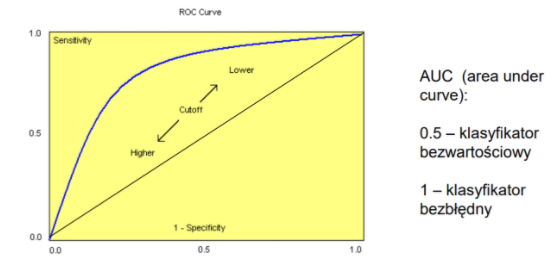
\includegraphics[width=0.7\linewidth]{S2.png}
	\caption{Krzywa ROC}
\end{figure}

Krzywa obrazująca czułość i specyficzność przy różnych wartościach progu predykcji. Im większe pole pod krzywą tym lepszy klasyfikator.  Na osi pionowej jest sensitivity a na poziomej specificity.

\subsubsection{Walidacja krzyżowa/Sprawdzian krzyżowy}

\begin{figure}[H]
	\centering
	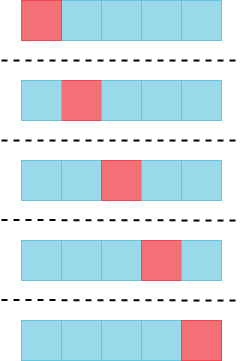
\includegraphics[width=0.2\linewidth]{S2_2.png}
	\caption{Krzywa ROC}
\end{figure}

Technika dokładnego testowania, Oryginalna próba jest dzielona na K podzbiorów. Następnie kolejno każdy z nich bierze się jako zbiór testowy, a pozostałe razem jako zbiór uczący i wykonuje analizę. Analiza jest więc wykonywana K razy. K rezultatów jest następnie uśrednianych (lub łączonych w inny sposób) w celu uzyskania jednego wyniku.

\subsubsection{Techniki dostrajania i wyboru modelu}

\begin{itemize}
	\item \textbf{Wybór optymalnych hiperparametrów modelu} - Każdy model ma inne parametry do dostrajania, np. funkcje aktywacji w sieciach neuronowych czy głębokość drzew w lasach losowych. Nie ma standardowej procedury wyboru, najczęściej trenuje się model dla różnych wartości parametru i dobiera ten dla którego wyszedł najlepszy wynik. Grid search i random search, gradient descent itd.
	\item \textbf{Zmiana długości uczenia i wczesne zatrzymanie} - Przy zbyt długim uczeniu, może wystąpić efekt przeuczenia, czyli zbyt dokładnego dopasowania do danych treningowych, aby temu zapobiec, należy odpowiednio wcześnie zatrzymać uczenie, np. w momencie kiedy błąd na zbiorze walidacyjnym zaczyna rosnąć
	\item \textbf{Redukcja wymiarowości cech} W niektórych przypadkach zmniejszenie liczby cech może polepszyć działanie modelu, poprzez zapobieganie przeuczaniu i poprawę zdolności do uogólniania
\end{itemize}






















